\documentclass[a4paper,parskip,11pt, DIV12]{scrreprt}
\usepackage[english]{babel} % Für Deutsch [english] zu [ngerman] ändern. 
\usepackage[utf8]{inputenc}
\usepackage[T1]{fontenc}
\usepackage{lmodern}
\usepackage{blindtext}
\usepackage{graphicx}
\usepackage{caption}
\usepackage{subcaption}
%\renewcommand{\familydefault}{\sfdefault}
%\usepackage{helvet}
\usepackage{fancyhdr}
\usepackage{amsmath}
\usepackage{mdwlist} %Benötigt für Abstände in Aufzählungen zu löschen
\usepackage{framed} %Rahmen um Objekte
\usepackage{floatflt} %Text neben Bildern
\usepackage{colortbl} % Tabellen einfärben
\usepackage{here}
\usepackage{calc}
\usepackage{hhline}
\usepackage{marginnote}
\usepackage{chngcntr}
\usepackage{tabularx}
\usepackage{titlesec} % Textüberschriften anpassen

% \titleformat{Überschriftenklasse}[Absatzformatierung]{Textformatierung} {Nummerierung}{Abstand zwischen Nummerierung und Überschriftentext}{Code vor der Überschrift}[Code nach der Überschrift]

% \titlespacing{Überschriftenklasse}{Linker Einzug}{Platz oberhalb}{Platz unterhalb}[rechter Einzug]

\titleformat{\chapter}{\LARGE\bfseries}{\thechapter\quad}{0pt}{}
\titleformat{\section}{\Large\bfseries}{\thesection\quad}{0pt}{}
\titleformat{\subsection}{\large\bfseries}{\thesubsection\quad}{0pt}{}
\titleformat{\subsubsection}{\normalsize\bfseries}{\thesubsubsection\quad}{0pt}{}

\titlespacing{\chapter}{0pt}{-2em}{6pt}
\titlespacing{\section}{0pt}{6pt}{-0.2em}
\titlespacing{\subsection}{0pt}{5pt}{-0.4em}
\titlespacing{\subsubsection}{0pt}{-0.3em}{-1em}

%\usepackage[singlespacing]{setspace}
%\usepackage[onehalfspacing]{setspace}

\usepackage[
			%includemp,				%marginalien in Textkörper einbeziehen
			%includeall,
			%showframe,				%zeigt rahmen zum debuggen		
			marginparwidth=25mm, 	%breite der marginalien
			marginparsep=5mm,		%abstand marginalien - text
			reversemarginpar,		%marginalien links statt rechts
			%left=50mm,				%abstand von Seitenraendern
%			top=25mm,				%
%			bottom=50mm,
			]{geometry}		

%Bibliographie- Einstellungen
\usepackage[babel,german=quotes]{csquotes}
\usepackage[
   backend=bibtex8, 
   natbib=true,
    style=numeric,
    sorting=none
]{biblatex}
\bibliography{Quelle}
%Fertig Bibliographie- Einstellungen

\usepackage{hyperref}

\begin{document}

\begin{titlepage}
\begin{figure}[h]
\hfill

\includegraphics[scale=0.04]{uzh}
\end{figure}
\vspace{1 cm}
\textbf{\begin{huge}Labreport solid-state physics
\end{huge}}\\
\noindent\rule{\textwidth}{1.1 pt} \\

\begin{Large}\textbf{Resistivitymeasurement of a HTSC-Metal}
\end{Large}\\ 
\normalsize 
\par
\begingroup
\leftskip 0 cm
\rightskip\leftskip
\textbf{Modul:}\\ Solid state physics PHY210 \\ \\
\textbf{Assistance:}\\ Oleh Ivashko ; oleh.ivashko@physik.uzh.ch \\ \\
\textbf{Student:}\\ S.Hochrein, H.Imboden, S.Buse\\ \\
\textbf{Date:}\\ 13.06.2017 \\ \\
\par
\endgroup
\clearpage

\end{titlepage}


%Start Layout
\pagestyle{fancy}
\fancyhead{} 
\fancyhead[R]{\small \leftmark}
\fancyhead[C]{\textbf{Solid state physics} } 
\fancyhead[L]{
\includegraphics[height=2\baselineskip]{uzh}}

\fancyfoot{}
\fancyfoot[R]{\small \thepage}
\fancyfoot[L]{}
\fancyfoot[C]{}
\renewcommand{\footrulewidth}{0.4pt} 

\addtolength{\headheight}{2\baselineskip}
\addtolength{\headheight}{0.6pt}


\renewcommand{\headrulewidth}{0.6pt}
\renewcommand{\footrulewidth}{0.4pt}
\fancypagestyle{plain}{				% plain redefinieren, damit wirklich alle seiten im gleichen stil sind (ausser titlepage)
\pagestyle{fancy}}

\renewcommand{\chaptermark}[1]{ \markboth{#1}{} } %Das aktuelle Kapitel soll nicht Gross geschriben und Nummeriertwerden

\counterwithout{figure}{chapter}
\counterwithout{table}{chapter}
\counterwithout{equation}{chapter}
%Ende Layout

\tableofcontents





\chapter{Introduction}
Superconductivity in metals and alloys is characterized by a sudden disappearance of resistance for temperatures lower than a certain transition temperature, $T_c$. Not all materials can become superconducting and if they do, the temperature at which they do is not the same for different materials. Some only become superconducting at less than 5K (Mercury for example) while some can still be superconducting above 130K (Hg-Ba-Ca-Cu-O). \\
In our experiment, YBa$_2$Cu$_3$O$_{7-\mathrm{\delta}}$ was used. This material has a transition temperature of around 92K.

\begin{figure}[H]
\centering
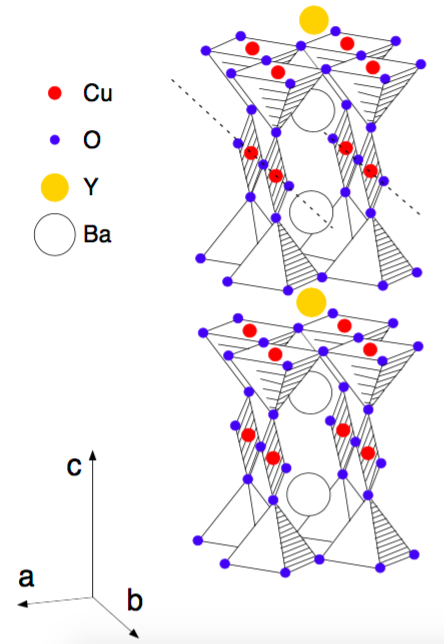
\includegraphics[width=6cm]{supercond.png}
\caption{Crystal structure of YBa$_2$Cu$_3$O$_{7-\mathrm{\delta}}$}
\end{figure}


\chapter{Experimental setup and Procedure}
The setup consists of four main parts \footnote{\url{http://www.physik.uzh.ch/data/peter/FestkoerperPhysik/InfoPraktFestkoerperphysik.shtml}}\\
\begin{itemize}
\item The specimen holder.\\
 This is where the superconductor was placed.\\ This container was equipped with connections for the temperature sensor, the heating, the resistance measurement and both current supply and voltage supply.\\
\item The cryostat.\\
This part serves to regulate the temperature. The sample is enclosed in a tube, which is submerged in liquid nitrogen. To keep the sample at a certain temperature, a heating foil is attached behind the sample. The foil will heat the sample, as more current is applied to it. This heating foil is needed, as liquid nitrogen has a constant temperature of around 77K at atmospheric pressure. \\
\item The vacuum system.\\
A vacuum of $2.8 \cdot 10^{-3}$mbar was created inside the tube. This vacuum helps to reduce the heat transfer between the probe and its surroundings, as heat is primarily exchanged through convection. With increasing vacuum, less convection can occur, as less air is inside the tube. 
\item The electromagnet.\\
The tip of the tube with the sample, including the cooling, was placed inside an electromagnet. The dependence of the resistance for different static magnetic fields could thus be measured.
\end{itemize}

~\\
  
Before measuring the resistance of our superconductor, the sample was cooled down to around 82K. The cooling (as well as the heating) was then cut out and the resistance was measured. The sample's temperature then increased slowly, as the surrounding room temperature was much higher. Thanks to the isolation created by the vacuum however, this temperature change was very slow. This allowed for a precise measurement of the transition temperature $T_c$.\\
To get the best possible measurement for the resistance, we used the so called four point measuring. The current supply is independent of the voltage metering. This allows for an undisturbed measuring of the voltage. 

\begin{figure}[H]
\centering
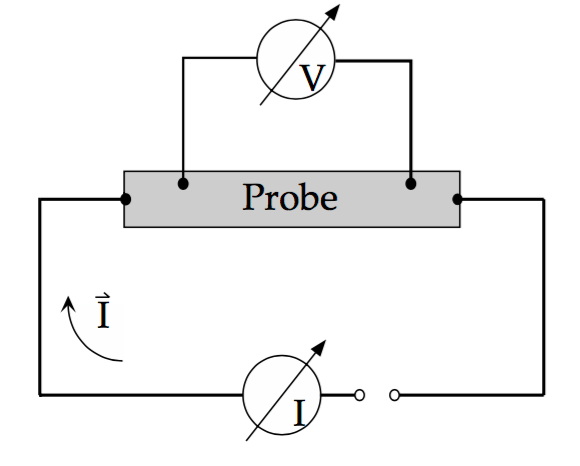
\includegraphics[width=7cm]{vierpunkt.png}
\caption{Illustration of the four-point measuring technique}
\end{figure}




\chapter{Results}
Hier kommen resultate
\begin{framed}
\begin{table}[H]
\centering
\renewcommand{\arraystretch}{1.2} % Abstandzwischen Zeilen
\setlength{\tabcolsep}{3mm} % Abstandzwischen Spalten
\footnotesize
\begin{tabular}{r|ccc}
$B[T]$ & 0 & 0.42 & 0.7 \\ 
\hline 
$T_{c} [K]$ & 94.3 $\pm$ 0.4 & 94.0 $\pm$ 0.4 & 94.1 $\pm$ 0.5 \\ 
\end{tabular}
\caption[]{Results}
\end{table} 
\end{framed}





\begin{figure}[H]
\centering
\includegraphics[scale=0.5]{Widerstand}
\caption[]{Measurement of the mean resistance.}
\end{figure}

\section{Questions}

1. Verhält sich wie ein Metall. Widerstand steigt mit der Temperatur.

2. Keine Magnetfeldabhängigkiet. Hall Effekt sorgt für Kräftegleichgewicht. Schwache Felder

3. Hauptidee Bericht

4. Kontaktspannung, richtungsabhängig


\chapter{Error calculus}


\section{Derivative}

Since the measurement more or less looks like a step-function one can get the error of $T_{c}$ by looking at the width of the derivative-curve. In an ideal case the derivative of a step-function would give a $\delta$-function which is localised in one point. Since the measured data has a lot of noise on top of the underling curve, we had to use the so called \emph{five-point-stencil method \footnote{\url{https://en.wikipedia.org/wiki/Five-point_stencil}}} to compute the derivative. Otherwise we wouldn't see the peak we are looking for. 

The \emph{five-point-stencil method} takes not only the next date point into account but also the 4 surrounding values. With this method we get a more smooth and useful curve. 

$$f'(x) \approx \frac{-f(x+2 h)+8 f(x+h)-8 f(x-h)+f(x-2h)}{12 h}$$

\begin{figure}[H]
\centering
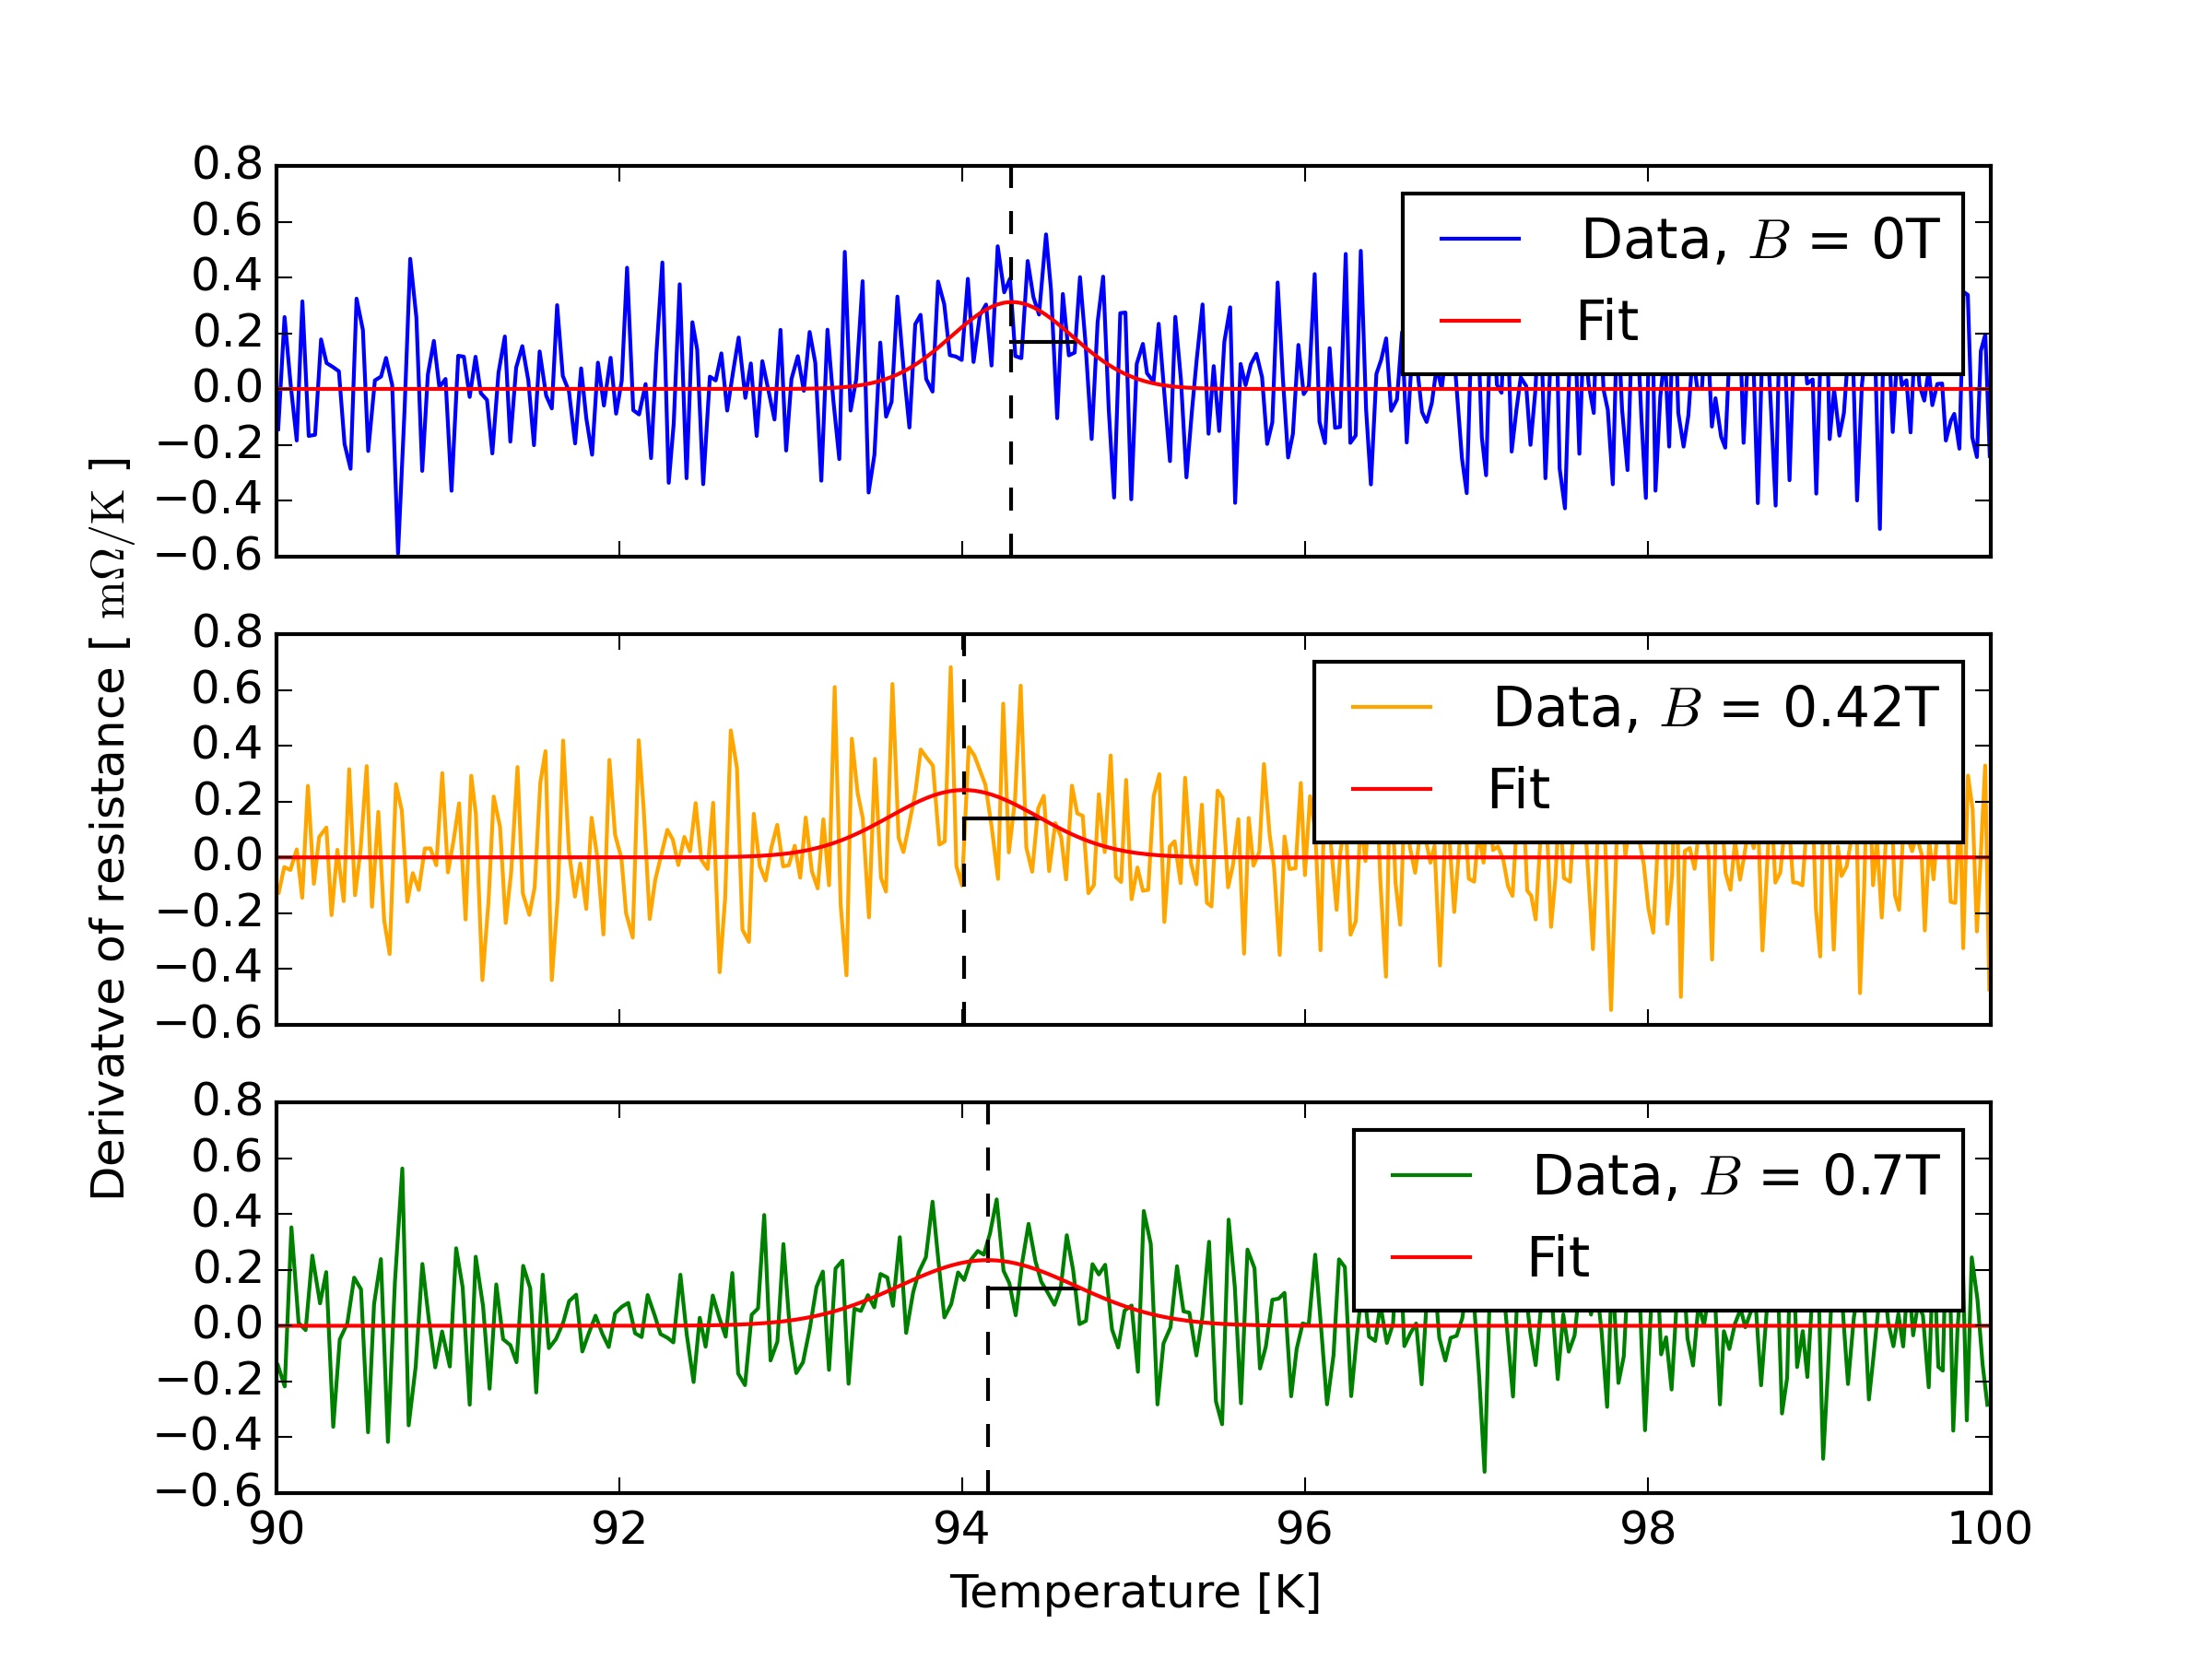
\includegraphics[scale=0.11]{Criticaltemperature3}
\caption[]{Derivative calculated using the five-point stencil method and considering the direct neighbours (h=1).  }
\end{figure}

\begin{figure}[H]
\centering
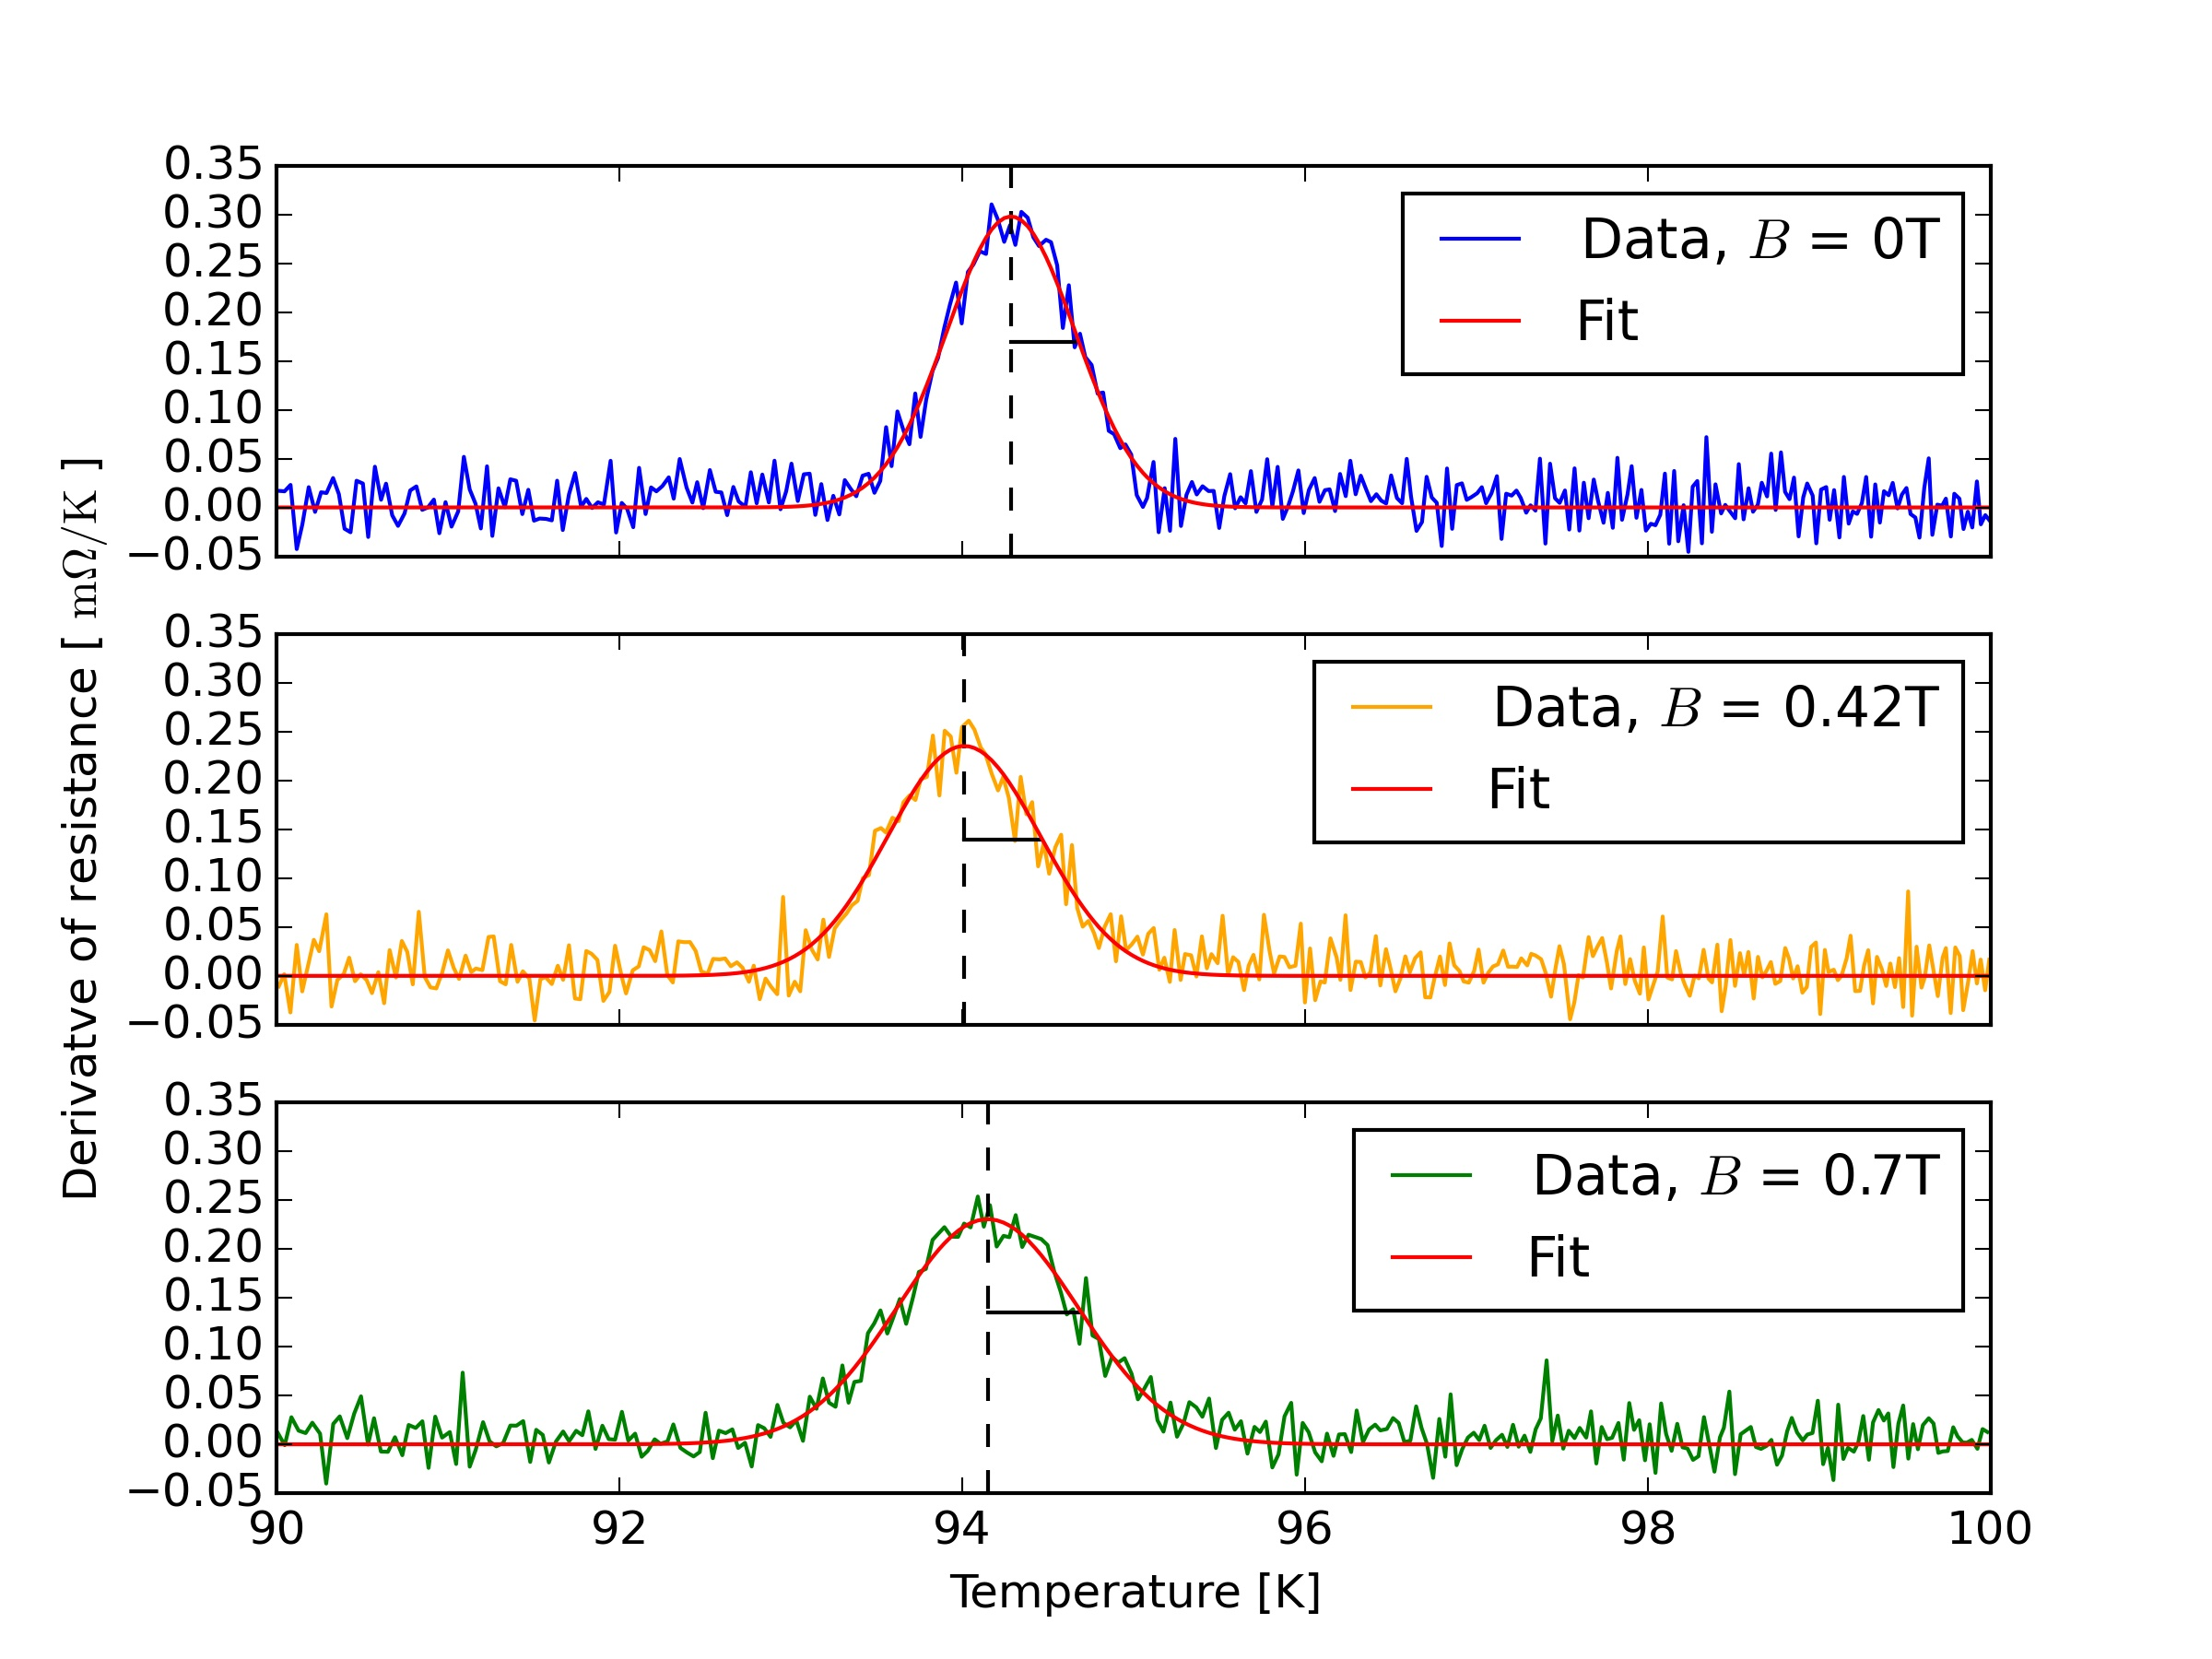
\includegraphics[scale=0.11]{Criticaltemperature2}
\caption[]{Derivative calculated with h=10.}
\end{figure}





\end{document}
